% В этом шаблоне используется класс spbau-diploma. Его можно найти и, если требуется, 
% поправить в файле spbau-diploma.cls
\documentclass{spbau-diploma}
\newcommand{\todo}{\textcolor{red}}

\begin{document}
% Год, город, название университета и факультета предопределены,
% но можно и поменять.
% Если англоязычная титульная страница не нужна, то ее можно просто удалить.
\filltitle{ru}{
    chair              = {Кафедра математических и информационных технологий},
    title              = {Решение задачи восстановления клональных деревьев репертуара антител с помощью данных парного иммуносеквенирования},
    % Здесь указывается тип работы. Возможные значения:
    %   coursework - Курсовая работа
    %   diploma - Диплом специалиста
    %   master - Диплом магистра
    %   bachelor - Диплом бакалавра
    type               = {master},
    position           = {студента},
    group              = 605,
    author             = {Черниговская Мария Александровна},
    supervisorPosition = {к.\,ф.-м.\,н., постдок \\Калифорнийского университета в Сан-Диего\\},
    supervisor         = {Сафонова Я.\,Ю.},
    reviewerPosition   = {\todo{??}\\},
    reviewer           = {Шугай М.\,А.},
    chairHeadPosition  = {д.\,ф.-м.\,н., профессор},
    chairHead          = {Омельченко А.\,В.},
    % university = {САНКТ-ПЕТЕРБУРГСКИЙ АКАДЕМИЧЕСКИЙ УНИВЕРСИТЕТ},
    % faculty = {Центр высшего образования},
    % city = {Санкт-Петербург},
    % year             = {2013}
}
\filltitle{en}{
    chair              = {Department of Mathematics and Information Technology},
    title              = {Clonal trees reconstruction of antibody repertoires using paired single cell sequencing data},
    author             = {Maria Chernigovskaya},
    supervisorPosition = {Ph.D., postdoc at UCSD\\},
    supervisor         = {Yana Safonova},
    reviewerPosition   = {\todo{??}\\},
    reviewer           = {Mikhail Shugay},
    chairHeadPosition  = {professor},
    chairHead          = {Alexander Omelchenko},
}
\maketitle
\tableofcontents

\section*{Реферат}

В работе описывается алгоритм  pairedAntEvolo, который позволяет анализировать данные парного иммуносеквенирования, полученные методом секвенирования одиночных клеток.
Алгоритм предназначен для разбиения репертуара B-клеток на клональные линии и восстановления эволюционных деревьев внутри каждой линии.
 \\

\textbf{Ключевые слова:} парное иммуносеквенирование, секвенирование одиночных клеток, клональные линии, клональные деревья, B-клетки, репертуар антител, созревание лимфоцитов, адаптивный иммунный ответ

% -------------------------------------------------------------------------------------------

\section{Введение}

% Какие-то вводные слова
Иммунная система защищает организм от заболеваний путем обнаружения патогенов — бактерий, вирусов, паразитов и других. 
Иммунная система умеет отличать патогены от биомолекул собственного организма и уничтожает их. 
Различают врожденный и приобретенный или адаптивный иммунитет. 
Задача врожденной иммунной системы дать быстрый неспицифичный ответ попадающим в организм патогенам. 
Адаптивная система дает специфичный иммунный ответ для каждого патогена и формирует иммунологическую память, запоминая специфичные для патогенных микроорганизмов антигены.


% Мы будем смотреть на В-клетки
Одним из важнейших элементов адаптивной иммунной системы являются В-клетки.
В-клетки экспрессируют специальные белки ---  антитела, которые циркулируют в крови и в лимфе.
Антитела распознают антигены -- поверхностные белки вирусов и бактерий -- связываются с ними и участвуют в их нейтрализации.


% Строение антитела 
Молекула антитела состоит из двух пар идентичных белков, которые называются тяжелые и легкие цепи.
Различают пять типов тяжелых цепей (альфа, гамма, дельта, эпсилон и мю) и два типа легких цепей (каппа и лямбда).
Вариабельные части тяжелой и легкой цепи образуют сайт связывания с антигеном и определяют специфичность антитела, то есть с каким именно антигеном будет связываться конкретное антитело.
В-клетки должны уметь синтезировать много различных антител, чтобы иммунная система могла бороться с огромным количеством потенциальных антигенов.
Так как количество возможных антигенов больше числа всех генов в ДНК, существуют специальные процессы, которые повышают разнообразие антител: VDJ-рекомбинация, спаривание тяжелой и легкой цепи, соматический гипермутагенез и клональная селекция.


\begin{figure}[h!]
    \centering
    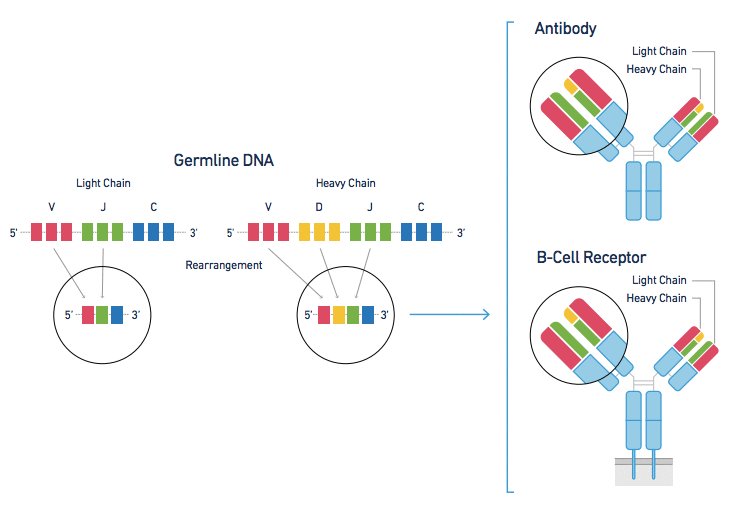
\includegraphics[width=.9\textwidth]{figures/10x_vdj_recombination.png}
    \caption{Схематичное описание VDJ-рекомбинации.
    В геноме присутствуют три группы генов: V, D и J гены, которые похожи внутри каждой группы.
    После рекомбинации тяжелая цепь содержит в себе по одному конкретному гену V, D и J, легкая цепь --- только V и J.
    Сперва рекомбинирует тяжелая цепь: на первом этапе рекомбинации вырезается случайное количество D-сегментов с конца и случайное количество J-сегментов с начала.
    На втором этапе вырезается случайное количество конечных V-сегментов и все D-сегменты, кроме последнего.
    На стыках V-D и D-J происходят случайные мутации и вставки.
    Лишние V- и J-гены затем вырезаются в процессе транскрипции.
    В итоге, оставшиеся V-, D и J- гены вместе с константной частью образуют ген тяжелой цепи иммуноглобулина.
    Получившаяся в ходе рекомбинации тяжелая цепь тестируется на продуктивность.
    Если цепь не работает, то рекомбинирует вторая аллель.
    Если обе цепи нефункциональны, то В-клетка погибает.
    Затем, аналогично тяжелой цепи, рекомбинирует легкая цепь.
    Если рекомбинация прошла успешно, то белки тяжелой и легкой цепь соединяются вместе и образуют антитело.
    сегменты.}
    \label{10x_vdj_recombination}
\end{figure}

% CDR3
VDJ-рекомбинация (рис.\ref{10x_vdj_recombination}) происходит во время дифференцировки гомопоэтической стволовой клетки в В-клетку и уникальным образом меняет ее геном. 
После VDJ-рекомбинации и последующей дифференцировки В-клетка покидает костный мозг.
Оставшиеся V-, D- и J- гены вместе с константной частью образуют ген иммуноглобулина, в котором присутствуют три определяющих комплементарность участка (англ. complementarity determining region, CDR). 
Эти участки кодируют часть белка, отвечающую за специфичность к антигену. 
CDR1 и CDR2 находятся внутри V-гена, а CDR3 захватывает V-ген, вставку (у тяжелых цепей вместе с D-геном) и J ген. 
CDR3  является самым вариабельным участком, и в гермлайне нет сегментов, которые могли бы его одназчно определить.     

% Откуда получаются деревья
Взрослые В-клетки циркулируют по крови и лимфе и посещают лимфоидные фолликулы вторичных лимфоидных органов, в которых концентрируются антигены, появившиеся в организме. 
После того, как В-клетка успешно свяжется с антигеном, она перемещается в герминальный центр и начинает делиться.
В получившихся клетках-клонах специальный фермент вносит соматические гипермутации в вариабельную часть антигена, чтобы улучшить связываемость антитела с антигеном.
На клетки действует негативный отбор, если их рецепторы нефункциональны или реагируют на аутоантигены.
\todo{Остальные} клетки стимулируются к дальнейшему делению и мутациям.
В результате такого эволюционного процесса образуются клональные семейства В-клеток. 


% Rep-seq vs single-cell
Существуют две технологии иммуносеквенирования, которые позволяют восстанавливать вариабельную часть генов иммуноглобулина.
Наиболее распространенное семейство технологий называется Rep-seq (Repertoire sequencing, ~\cite{pmid22043864}), которое позволяет с очень высокой точностью определить частоты антител в образце.
(\todo{Что-то написать про саму технологию(??)
В целом, это обычное секвенирование кДНК с правильно подобранными праймерами, которые садятся на консервативный кусок в начало V-гена})
Недостаток Rep-seq технологий --- в процессе секвенирования теряется важная информация, какие тяжелые и легкие цепи образовывали вместе антитело.
Не так давно появилась технология, которая позволяет секвенировать РНК антител одиночных клеток и сохранять информацию о парности цепей. 
К сожалению, на текущий момент не существует общепринятого и стабильного протокола, однако коммерческая компания 10х genomics является лидером по качеству парных данных.


% Цель работы
Целью данной работы является анализ реальных данных парного иммуносеквенирования и разработка метода восстановления клональных деревьев с помощью таких данных.



% -------------------------------------------------------------------------------------------

\subsection{Мотивация}

% Репертуар имеет структуру! Это не просто множество, а дерево
Большинство исследований (\cite{warren2013high},~\cite{jackson2014human},~\cite{logan2011high}) рассматривает репертуар как множество антител, однако клональные деревья позволяют использовать дополнительную информацию о эволюционнм процессе гипермутаций ~\cite{miho2017fundamental}.
При иммунном ответе на антиген В-клетки, связанные с этим антигеном, интенсивно делятся, и важные антитела можно увидеть в самых больших деревьях.

% Хорошо смотреть на тайм серии
Клональные деревьев позволяют изучать динамику иммунного ответа по данным временных серий ~\cite{hoehn2015dynamics}.
Также можно изучать, какие именно мутации оказались самыми полезными и привели к наибольшему распространению клона.

\todo{Есть статья, в которой клональные деревья дали больше чем Rep-seq??}


% Зачем строить парные деревья 
\todo{Зачем строить парные деревья??}
Для того, чтобы синтезировать антитело как лекарство, необходимо знать последовательности легкой и тяжелой цепи, потому что они обе отвечают за специфичность к антигену. 
(Не отвечает на вопрос, зачем строить именно деревья)
А еще лучше смотреть на парный репертуар, чтобы не строить мнимые деревья, потому что есть allelic inclusion. 
(строим, чтобы изучать allelic inclusion?)

% -------------------------------------------------------------------------------------------

\subsection{Постановка задачи}

\textbf{Биологическая постановка задачи}: дан репертуар антител, который был получен с помощью технологии секвенирования одиночных клеток. 
Необходимо восстановить эволюционный процесс, то есть
\begin{itemize}
    \item  разбить репертуар на клональные линии;
    \item  внутри каждой клональной линии восстановить отношения <<ребенок-родитель>> между В-клеток. 
\end{itemize}

\textbf{Вычислительная постановка задачи}: дан набор строк. 
Каждая строка является вариабельной частью легкой или тяжелой цепи некоторых иммуноглобулинов. 
Строка имеет клеточный баркод, причем цепи, которые относятся к одной клетке имеют одинаковые баркоды, а к разным клеткам --- разные баркоды. 
Необходимо восстановить лес на подмножествах строк удовлетворяющий требованиям
\begin{itemize}
    \item строки с одинаковым клеточным баркодам соответствуют В-клетке;
    \item вершина дерева соответствует всем В-клеткам, которые имеют одинаковые цепи;
    \item вершины внутри одного дерева соответствуют В-клеткам, которые имеют общего предка;
    \item ребра между вершинами соответствуют отношениям <<ребенок-родитель>> между клетками;
    \item получившееся дерево соответствует принципу минимальной эволюции. 
\end{itemize}

Задача решается в условиях известного референса, в котором содержатся известные варианты V и J сегментов (гермлайн). 
С помощью выравнивания на гермлайн мы можем узнать, какие V- и J-гены содержит каждая последовательность. 
Эта информация позволяет проаннотировать последовательности, то есть найти соматические гипермутации.

% -------------------------------------------------------------------------------------------

\subsection{Существующие решения}

% Для одной цепи
Задача разбиения репертуара антител на клональные линии хорошо изучена для Rep-seq данных~\cite{davidsen2018benchmarking}, однако для построения клональных деревьев еще не разработан общепринятый подход. 
Некоторые авторы~\cite{hoehn2016diversity} сводят задачу к филогенетической, хотя такое решение некорректно по двум причинам. 
Во-первых, филогенетические алгоритмы не учитывают структуру последовательностей, и что общий предок всех клеток из одной клональной линии должен быть составлен из генов гермлайна. 
Во-вторых, филогенетические алгоритмы подразумевают, что все наблюдаемые последовательности являются листьями эволюционного дерева. 
Однако есть и принципиально другой подход~\cite{horns2016lineage}, который основан на множественном выравнивании похожих последовательностей. 

% Для двух цепей (bracer)
В сентябре $2017$ года вышла статья~\cite{lindeman2017bracer}, в которой описан BraCeR --- алгоритм построения клональных деревьев для данных парного иммуносеквенирования. 
Алгоритм состоит из следующих шагов:
\begin{enumerate}
    \item Кластеризация похожих цепей: \\
    Две цепи считаются похожими, если они аннотированы одинаковыми V- и J-генами, их CDR3 имеют одинаковую длину и находятся на расстоянии не больше $0.2$. 
    Расстояние между последовательностями CDR3 (взято из статьи~\cite{yaari2013models}) основывается на распределении соматических гипермутаций в разных $5$-мерах.
    \item Построение клональных линий: \\
    Две клетки принадлежат одной клональной линии, если они имеют хотя бы одну похожую тяжелую цепь и хотя бы одну похожую легкую цепь. 
    \item Построение клональных деревьев:  \\
    Клональные деревья строятся с помощью филогенетического алгоритма PHYLIP. 
\end{enumerate}

BraCeR имеет несколько недостатков:
\begin{itemize}
    \item Основывается на филогенетическом алгоритме.
    \item Работает только для небольшого числа клеток (около $100$) из-за особенностей реализации. При этом современные технологии парного иммуносеквенирования производят данные для нескольких тысяч клеток.
    \item Не удалось воспроизвести результаты статьи. \todo{Попробовать еще раз}
\end{itemize}

% -------------------------------------------------------------------------------------------

\section{Анализ реальных данных}

\subsection{Описание технологии парного иммуносеквенирования на примере данных 10х}

% Описание технологии
На текущий момент компания 10x genomics~\cite{pmid28091601} лидирует в производстве парных данных.
Их технология секвенирования одиночных иммунных клеток (рис.\ref{10x_pipeline}) позволяет с высокой точностью обработать от 100 до 10000 клеток в одном образце.
Для того, чтобы запомнить информацию о том, какие цепи экспрессирует конкретная клетка, используют клеточные и молекулярные баркоды (рис.\ref{10x_barcodes}).
Клеточные баркоды позволяют отметить последовательности, которые относятся к одной клетке.
Молекулярные баркоды нужны для того, чтобы идентифицировать последовательности после амплификации.
Помеченные двумя баркодами последовательности секвенируют с помощью парных ридов (150 нуклеотидов), которые затем собираются в контиги с помощью разработанного в компании инструмента CellRanger VDJ.
Затем происходит аннотация --- контиги выравниваются на базу известных V, D, J сегментов (гермлайн), и последовательности с плохим выравниванием отфильтровываются.
Для оставшихся последовательностей определяется лучшее выравнивание на V и J сегменты.
В конечном итоге получается набор последовательностей цепей иммуноглобулинов с клеточным баркодом и предполагаемыми V и J сегментами, которые были выбраны в ходе VDJ-рекомбинации.

\begin{figure}[h!]
    \centering
    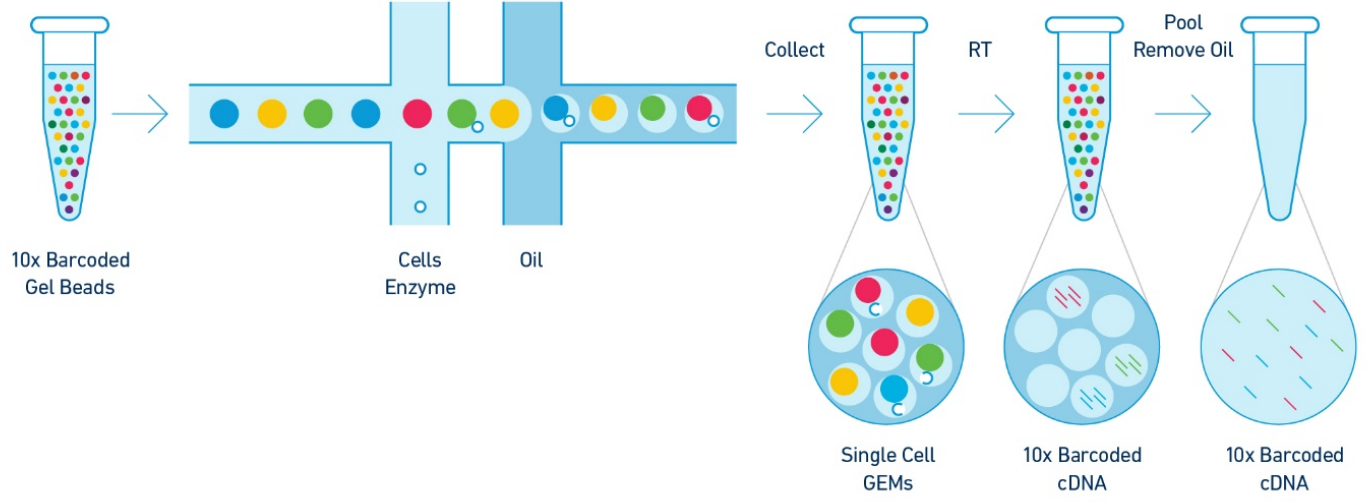
\includegraphics[width=.9\textwidth]{figures/10x_pipeline.png}
    \caption{Описание технологии 10x genomics VDJ: На вход поступает клеточная суспензия определенной плотности.
    Клетки вместе с реагентами реакции проходят через микрофлюидный (микрогидродинамический) канал, смешиваются с гелевыми шариками и лизисным буфером из другого канала и формируют капли, изолированные друг от друга маслом.
    На поверхности гелевых шариков находятся баркодированные олигонуклеотиды.
    Внутри капли за секунды происходит лизис клетки, и содержимое клетки, в том числе молекулы матричной РНК, оказывается внутри капли.
    Молекулы мРНК гибридизуются с олигонуклеотидами на поверхности шариков, и затем внутри капли происходит обратная транскрипция молекул мРНК в молекулы кДНК.
    Затем капли <<лопаются>>, полученная библиотека кДНК амплифицируется с помощью ПЦР и отправляется на секвенирование}
    \label{10x_pipeline}
\end{figure}

\begin{figure}[h!]
    \centering
    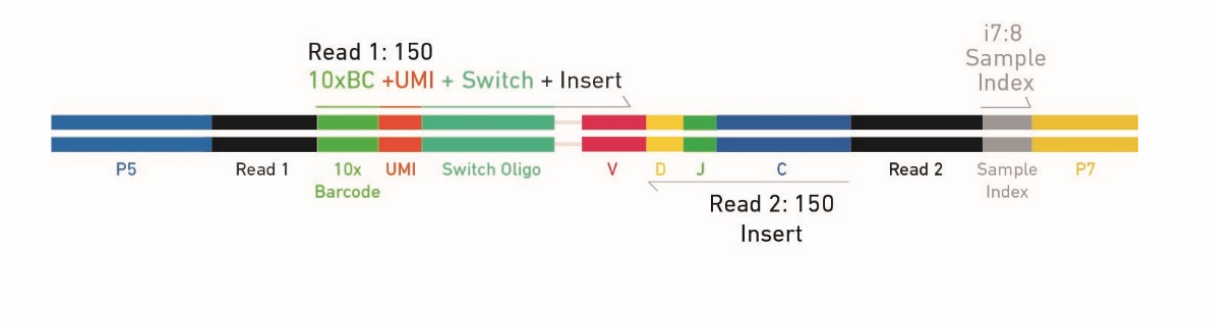
\includegraphics[width=.9\textwidth]{figures/10x_barcodes.png}
    \caption{Структура библиотеки: левый рид покрывает клеточный (16 нуклеотидов) и молекулярный (10 нуклеотидов) баркод.
    Оба рида являются стандартными парными ридами для технологии Illumina и используются для того, чтобы покрыть вставку.}

    \label{10x_barcodes}
\end{figure}

% Сколько цепей может экспрессировать В-клетка
Известно, что при созревании В-лимфоцитов происходит аллельное исключение, то есть успешная VDJ-рекомбинация гена \todo{локуса?}, который кодирует тяжелую цепь иммуноглобулина на одной хромосоме, блокирует  рекомбинацию в гомологичной хромосоме.
Однако существует исследование~\cite{barreto2000frequency}, в котором показано, что у здоровых мышей в $1$ случае из $10000$ может происходить одновременная экспрессия обеих тяжелых цепей в IgM+ В-клетках селезенки.
Авторы статьи предложили несколько моделей, которые могли бы объяснить данное явление, но пока эти гипотезы не подтверждены.
У человека неизветны случаи, в которых В-клетки экспрессируют несколько тяжелых цепей, но есть исследование, в котором показали, что $30\%$ клеток гибридомы (гибридная клеточная линия, которая получена в результате слияния B-лимфоцитов из селезенки иммунизированного животного и опухолевых клеток миеломы) имели дополнительные тяжелые и легкие цепи.
Причем  $1.1\%$ клеток имели дополнительную легкую цепь, а $2.2\%$ --- дополнительную тяжелую и легкую цепь.
На текущий момент проведено множество исследований (~\cite{pelanda2014dual}, ~\cite{casellas2007igkappa}, ~\cite{liu2005receptor}, ~\cite{fraser2015immunoglobulin}), которые подтверждают, что В-клетки могут экспрессировать две легкие цепи как одного, так и разных типов.
Большинство таких В-клеток экспрессируют две легкие каппа-цепи, но редко могут экспрессировать две лямбда-цепи и цепи разных типов.
Одно экспрессируемое антитело может быть аутореактивным, а второе \todo{нормальным}, которое позволит В-клетке обмануть негативную селекцию, созреть, активироваться и дифференцироваться.
Считается~\cite{dekosky2015depth}, что В-клетки  с двумя различными легкими цепями встречаются примерно в $1\%$ случаях.


% Что мы ожидаем от данных
Таким образом, мы ожидаем увидеть в парных данных, что большинство В-клеток экспрессируют одну легкую и одну тяжелую цепь или (редко) одну тяжелую и две легких цепи.
Мы можем увидеть не все цепи в данных секвенирования, так мы можем не захватить молекулы РНК при подготовке библиотеки.
Поэтому мы также ожидаем увидеть в данных клетки, которые имеют только легкую или только тяжелую цепь.
Клетки, у которых просеквенирован нестандартный набор цепей, например несколько тяжелых и больше двух легких цепей, скорее всего являются артефактом секвенирования и получились в результате коллизии, при которой больше одной клетки попадали в каплю с молекулярными баркодами.
10х genomics утверждают~\cite{10x_manual}, что вероятность коллизии зависит от концентрации клеток в образце, и варьируется от $0.4\%$ до $7.6\%$.



\subsection{Анализ публичных В-клеточных датасетов 10х}

% Описание датасетов
Для того, чтобы изучить специфику парных данных 10x, были проанализированы публичные В-клеточные датасеты~\cite{10x_datasets}: 
\begin{enumerate}
    \item CD19 --- B-клетки с маркером CD19, которые были выделены из мононуклеарных клеток периферической крови здоровых доноров.
    Так как этот вид клеток экспрессирует небольшое количество РНК, библиотека прошла целевое обогащение;
    \item GM12878 --- В-лимфобластоидная клеточная линия с высоким уровнем транскрипции иммуноглобулинов;
    \item NSCLC --- целевое обогащение иммуноглобулинов B-клеток, которые были получены во время свежего хирургического удаления немелкоклеточного рака легкого.
\end{enumerate}

% Баги в аннотации
Помимо стандартных типов цепей иммуноглобулинов --- тяжелая, легкая каппа и легкая лямбда, последовательности аннотируют еще одним типом --- мультицепь.
Мультицепь --- это последовательность, которая выравнивается на гены разных типов, например V ген выравнивается на каппу-цепь, а J ген на лямбду.
На практике мы наблюдаем, что в мультицепи попадают последовательности, которые были неправильно проаннотированы.
Например, последовательность TGACGGCAGTGAACGC\-1\_contig\_4 из датасета CD19 (подтверждена $83$ молекулярными баркодами) в аннотации 10х имеет IGLV3-21 и IGHJ6 гены, хотя IgBLAST, который считается золотым стандартом аннотации иммуных последовательностей, проаннотировал этот контиг генами IGLV3-21*02 и IGLJ1*01 с хорошим качеством выравнивания.
Также в аннотациях 10х встречаются последовательности, которые содержат одновременно T- и В-клеточные гены, но на самом деле они содержат лишь какие-то подпоследовательности генов иммуноглобулинов (рис.\ref{IgBLAST_multi}).
Мы предполагаем, что это объясняется тем, что в парные данные также попадает мусорная РНК, которая транскрибируется из иммунного локуса, и 10х плохо отфильтровывает такие контиги.


\begin{figure}[h!]
  \centering
  \begin{subfigure}{\linewidth}
    \centering
    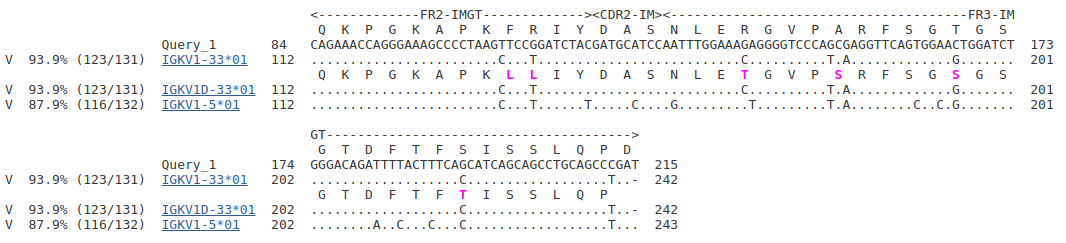
\includegraphics[width=1\textwidth]{figures/IgBLAST_bcr.png}
    \caption{Аннотация контига IgBlAST с выравниванием на базу В-клеточных генов иммуноглобулинов}
  \end{subfigure}

  \begin{subfigure}{\linewidth}
    \centering
    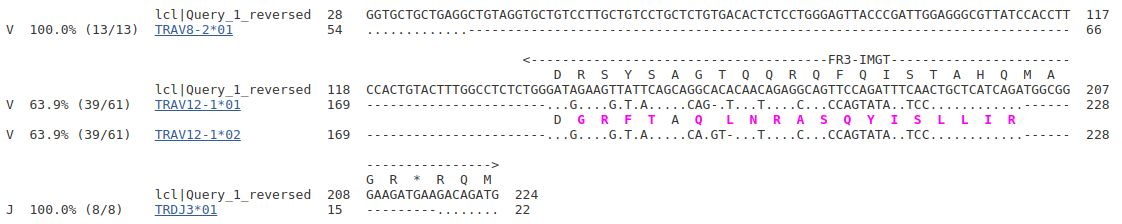
\includegraphics[width=1\textwidth]{figures/IgBLAST_tcr.png}
    \caption{Аннотация контига IgBlAST с выравниванием на базу Т-клеточных генов иммуноглобулинов}
  \end{subfigure}  
  \caption{Пример последовательности, которая проаннотирована 10х как мультицепь с Т-клеточным геном TRAJ22 и В-клеточными геном IGKV2D-28 (контиг GAACATCTCGGCGGTT\-1\_contig\_4 из датасета CD19, подтвержден $65$ молекулярными баркодами).
  Из аннотации IgBLAST видно, что последовательность плохо выравнивается на обе базы генов, а также в лучших выравниваниях не содержатся гены, которые были указаны в аннотации 10х.}

  \label{IgBLAST_multi}
\end{figure}  


% Сравнение 10х и IgBLAST
Чтобы проверить точность аннотации данных с помощью 10х, мы сравнили ее с IgBLAST.
Во всех датасетах мы оставили только те контиги, которые относятся к иммуноглобулинам и в 10х аннотации которых указано, что эти контиги с высокой достоверностью являются цепями, а не мусором. 
Затем мы проаннотировали эти цепи с помощью IgBLAST. 
Из таблицы~\ref{10x_vs_IgBLAST} видно, что большой процент цепей были отфильтрованы, потому что они не выровнялись на базу генов.
Также среди отфильтрованных цепей оказалась все мультицепи, что подтверждает нашу гипотезу о том, что это не особый тип цепей, а не отфильтрованный мусор. 
Для оставшихся последовательностей мы посчитали, сколько из них проаннотированы одинаковыми V- и J-генами в обеих аннотациях (10х не учитывает разные аллели V- и J-генов, поэтому нам пришлось считать совпадения генов без учетов аллельных вариаций). 
Оказалось, что аннотации не совпадают в $10-20\%$ случаях для V-генов и в $1-4\%$ для J-генов. 
Этот результат согласовывается с тем, что V-гены длиннее (примерно $300$ нуклеотидов)  и их больше ($135$ генов всех типов), чем J-генов ($15$ генов всех типов, длина варьируется от $46$ до $63$ нуклеотидов).
Мы считаем, что это очень большой процент ошибок для аннотатора иммунных последовательностей.

Далее используются только цепи, оставшиеся после фильтрации IgBLAST.  

\begin{table}[h]
\centering
\begin{tabular}{|l|c|c|c|}
\hline
                                               & \multicolumn{1}{c|}{\textbf{CD19}} & \multicolumn{1}{c|}{\textbf{GM12878}} & \multicolumn{1}{c|}{\textbf{NSCLC}} \\ \hline
\multicolumn{4}{|c|}{\textbf{Исходная аннотация 10х}}                                                                                                             \\ \hline
\# цепей                                       & 31486                              & 2671                                  & 7509                                \\ \hline
\% мультицепей                                 & 23,78\%                            & 16,74\%                               & 12,73\%                             \\ \hline
\multicolumn{4}{|c|}{\textbf{Аннотация с помощью IgBLAST}}                                                                                                       \\ \hline
\% отфильтрованных цепей                       & 30,39\%                            & 17,86\%                               & 35,62\%                             \\ \hline
\% цепей с совпавшими аннотациями V-генов      & 82.53\%                            & 91.56\%                               & 79.43\%                             \\ \hline
\% цепей с совпавшими аннотациями J-генов      & 98.37\%                            & 99.41\%                               & 96.07\%                             \\ \hline
\% цепей с совпавшими аннотациями V- и J-генов & 81.25\%                            & 91.56\%                               & 76.58\%                             \\ \hline
\end{tabular}
\caption{Сравнение аннотации 10х и IgBLAST}
\label{10x_vs_IgBLAST}
\end{table}

% Статы по количеству цепей в клетке
Мы проверили, похожи ли частоты клеток с разным количеством цепей (таблица~\ref{stats_nchains}) на те, которые описывались ранее в статьях.
Клетки, у которых количество цепей больше четырех, скорее всего являются артефактами баркодных коллизий, причем клетки с пятью и более цепями содержатся только в датасете CD19, который примерно в $10$ раз больше двух других.
Также из таблицы видно, что процент клеток, которые экспрессируют три \todo{продуктивные} цепи противоречит нашим ожиданиям (должно быть меньше $1\%$).

% Точно разные цепи?
Для того, чтобы подтвердить, что это действительно разные цепи, а не артефакты технологии секвенирования и ПЦР, мы построили гистограмму расстояний (рис.~\ref{d_distribution}) между двумя цепями одного типа, которые находятся в клетке.
Расстояние было выбрано таким образом, чтобы значение $0$ соответствовало идентичным цепям, а отрицательное --- различающимся последовательностям, причем модуль расстояния не меньше количества мисматчей между последовательностями.
Из рисунка видно, что в среднем две кратные цепи отличаются не меньше, чем на $50-75$ нуклеотидов \todo{Почему мы считаем, что это много? }


\begin{table}[h!]
\centering
\begin{tabular}{|l|c|c|c|c|c|c|c|}
\hline
        & \textbf{1 цепь} & \textbf{2 цепи} & \textbf{3 цепи} & \textbf{4 цепи} & \textbf{5 цепей} & \textbf{6 цепей} & \textbf{\textgreater{}6 цепей} \\ \hline
CD19    & 22.67\%         & 63.26\%         & 10.53\%         & 2.7\%           & 0.69\%           & 0.14\%           & 0.01\%                         \\ \hline
GM12878 & 17.51\%         & 56.80\%         & 21.66\%         & 4.03\%          & 0.00\%           & 0.00\%           & 0.00\%                         \\ \hline
NSCLC   & 51.26\%         & 46.55\%         & 2.02\%          & 0.17\%          & 0.00\%           & 0.00\%           & 0.00\%                         \\ \hline
\end{tabular}
\caption{Процентное соотношение клеток по количеству \todo{productive (продуктивных?)} цепей}
\label{stats_nchains}
\end{table}

 
\begin{figure}[h]
    \centering
    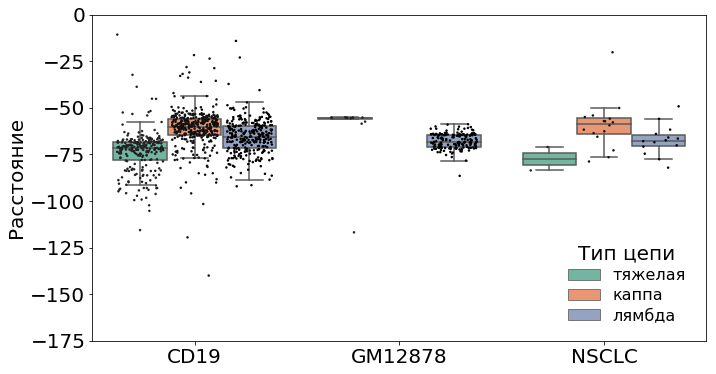
\includegraphics[width=1.\textwidth]{figures/d_distribution.png}
    \caption{Распределение расстояния между кратными цепями в клетках, которые содержат три \todo{продуктивные (productive)} цепи.  
    В качестве метрики было взято расстояние редактирования со следующими штрафами: $0$ за совпадение, $-1$ за несовпадение, $-0.5$ за открытие гэпа и $-0.1$ за его продолжение.}
    \label{d_distribution}
\end{figure}

   
   
   
Таким образом, парные данные 10х обладают следующими особенностями:
\begin{itemize}
    \item в данных встречаются последовательности, которые не являются цепями антител;
    \item неточная аннотация;
    \item количество клеток с тремя продуктивными цепями не соответствует остальным статьям.
\end{itemize}


% -------------------------------------------------------------------------------------------

\section{Симулятор парных данных}

~\cite{safonova2015igsimulator}

Мы сделали симулятор парных данных, потому что \\
1 не можем нормально бенчмаркать на реальных данных \\
2 на реальных данных мы не видим деревьев по тяжелым цепям \\
3 данные 10х странные \\


Каким частотам мы верим? 10x или~\cite{dekosky2015depth}.
Должна ли дополнительная цепь мутировать? Или отбор идет только по одному антителу?



% -------------------------------------------------------------------------------------------

\section{Описание алгоритма}

\subsection{Описание алгоритма AntEvolo}

\subsection{Модификация алгоритма AntEvolo}

\subsection{Описание алгоритма pairedAntEvolo}



% -------------------------------------------------------------------------------------------

\section{Экспериментальные результаты}

\subsection{Симулированные данные}

\subsection{Реальные данные}




% У заключения нет номера главы
\section*{Заключение}

\bibliographystyle{ugost2008ls}
\bibliography{diploma.bib}
\end{document}
